\chapter{Звук, квантовые осцилляторы и второй закон}

\lectureoverview{Второй закон — конечная цель, но путь к ней готовят два конкретных расчёта. Скорость звука показывает, как термодинамические производные превращаются в наблюдаемое движение. Затем гармонический осциллятор выявляет несостоятельность классического равнораспределения для жёстких степеней свободы и показывает, как квантовая механика включает моды по одной. В конце мы вернёмся к кажущемуся противоречию между обратимой микроскопической динамикой и возрастанием энтропии, используя поток в фазовом пространстве, огрубление, хаос и возвраты, чтобы сформулировать второй закон как закон, выполняющийся с подавляющей вероятностью, а не как механический запрет без исключений.}

\section{Обещание относительно второго закона}

Центральную проблему легко сформулировать и трудно объяснить. Ньютоновские уравнения обратимы: если допустима некоторая микроскопическая история, то допустима и история, обращённая по времени. Тем не менее второй закон утверждает, что макроскопические процессы имеют предпочтительное направление, характеризуемое энтропией, которая обычно возрастает. Мы ещё вернёмся к этому противоречию, но не сразу. Сначала лучше увидеть, как статистическая механика даёт конкретную информацию, а затем встретить, в рамках элементарного расчёта, историческую загадку, которая вынудила классическую физику уступить место квантовой.

Первый пример численный и намеренно грубый: оценить скорость звука в разрежённом газе. Второй точен в рамках своих предпосылок: вычислить среднюю энергию гармонического осциллятора в тепловой ванне. Осциллятор приведёт нас от равнораспределения к квантованным уровням энергии, от одной моды к бесконечно многим модам и, наконец, обратно к вопросу о том, что значит для многочастичной системы забывать своё начальное состояние.

\section{Молекулярный масштаб скорости звука}

Представьте себе небольшое локальное повышение плотности в разрежённом газе. Оно расплывается, потому что молекулы уходят из более плотной области, так что скорость его распространения должна быть сравнима с молекулярной скоростью. Равнораспределение даёт кинетическую энергию одной молекулы, \begin{equation}
 \frac{3}{2}k_B T
 =\frac{1}{2}m\expect{v^2},
 \qquad
 \expect{v^2}=\frac{3k_B T}{m}.
 \label{eq:sm7-molecular-speed}
\end{equation} Здесь температура отсчитывается от абсолютного нуля, и \(k_B\) восстановлена, потому что нам нужны лабораторные единицы. Этот довод — лишь оценка масштаба: среднеквадратичная молекулярная скорость сама по себе не является скоростью коллективной звуковой волны.

Более систематический вывод рассматривает малый элемент газа. Неравные давления на противоположных гранях создают результирующую силу, а его ускорение обратно пропорционально массовой плотности. Результат имеет вид \begin{equation}
 c_s^2=
 \left(\frac{\partial P}{\partial \rho_m}\right)_{\cal C},
 \qquad
 \rho_m=m\rho,
 \label{eq:sm7-sound-general}
\end{equation} где \(\rho\) — численная плотность, а индекс \({\cal C}\) задаёт термодинамическое условие, которому следует возмущение. Вычисление на доске использует \begin{equation}
 P=\rho k_B T
 \quad\Longrightarrow\quad
 \frac{1}{m}
 \left(\frac{\partial P}{\partial\rho}\right)_T
 =\frac{k_B T}{m}.
 \label{eq:sm7-sound-isothermal}
\end{equation} Это изотермическая оценка скорости звука. Она отличается от \eqref{eq:sm7-molecular-speed} множителем \(3\) в квадрате скорости, или \(\sqrt{3}\) в самой скорости.

\begin{figure}[t]
\centering
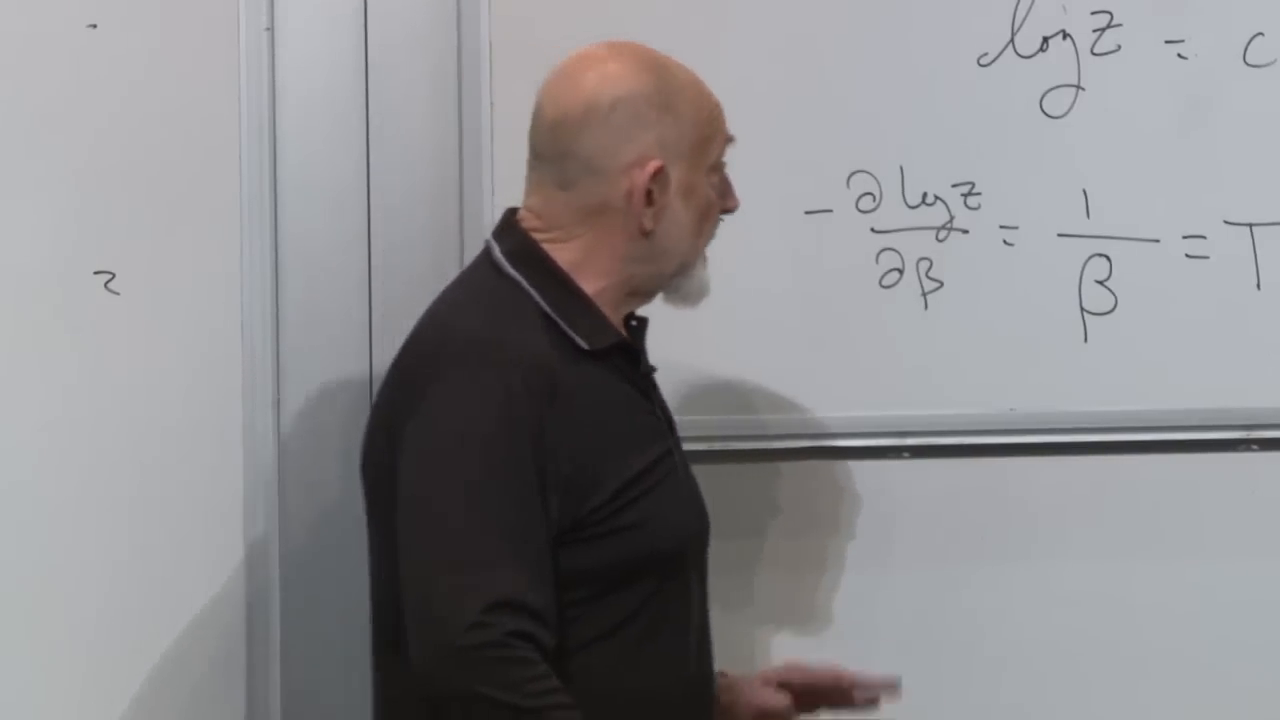
\includegraphics[width=0.90\textwidth]{lecture_07_figure_02.png}
\caption{Вместе показаны оценка по молекулярной скорости, производная давления и подстановка для идеального газа.}
\lectureframe{00:08:55}
\end{figure}

Есть важное уточнение. Звуковая волна малой амплитуды обычно сжимает и разрежает газ быстрее, чем тепло успевает перетекать между соседними элементами. Поэтому локальное движение приблизительно адиабатично, а не изотермично:
\begin{equation}
 c_s^2=
 \left(\frac{\partial P}{\partial\rho_m}\right)_S.
 \label{eq:sm7-sound-adiabatic}
\end{equation}
Для идеального газа с адиабатическим показателем \(\gamma\),
\begin{equation}
 P\rho_m^{-\gamma}=\text{constant},
 \qquad
 c_s^2=\gamma\frac{P}{\rho_m}
       =\gamma\frac{k_B T}{m}.
 \label{eq:sm7-sound-ideal-adiabatic}
\end{equation}
Для двухатомного воздуха при комнатной температуре \(\gamma\simeq 7/5\). Таким образом, расчёт при фиксированной температуре даёт полезную первую оценку, тогда как адиабатическая производная даёт физически правильное уточнение.

Используя грубые значения
\begin{equation}
\begin{aligned}
 k_B&\simeq1.3\times10^{-23}\ {\rm J\,K^{-1}},
 &T&\simeq300\ {\rm K},\\
 m_{\rm air}&\simeq4\times10^{-26}\ {\rm kg}.&&
\end{aligned}
 \label{eq:sm7-air-data}
\end{equation}
получаем, что молекулярная оценка составляет примерно \(500\ {\rm m\,s^{-1}}\). Температура здесь должна быть абсолютной температурой в кельвинах, а не шкалой со смещённым нулём, такой как шкала Фаренгейта. Привычная скорость звука имеет порядок \(300\ {\rm m\,s^{-1}}\), а адиабатическая формула идеального газа даёт при комнатной температуре около \(340\ {\rm m\,s^{-1}}\). Следовательно, грубый расчёт действительно нашёл правильный физический масштаб.

\begin{figure}[t]
\centering
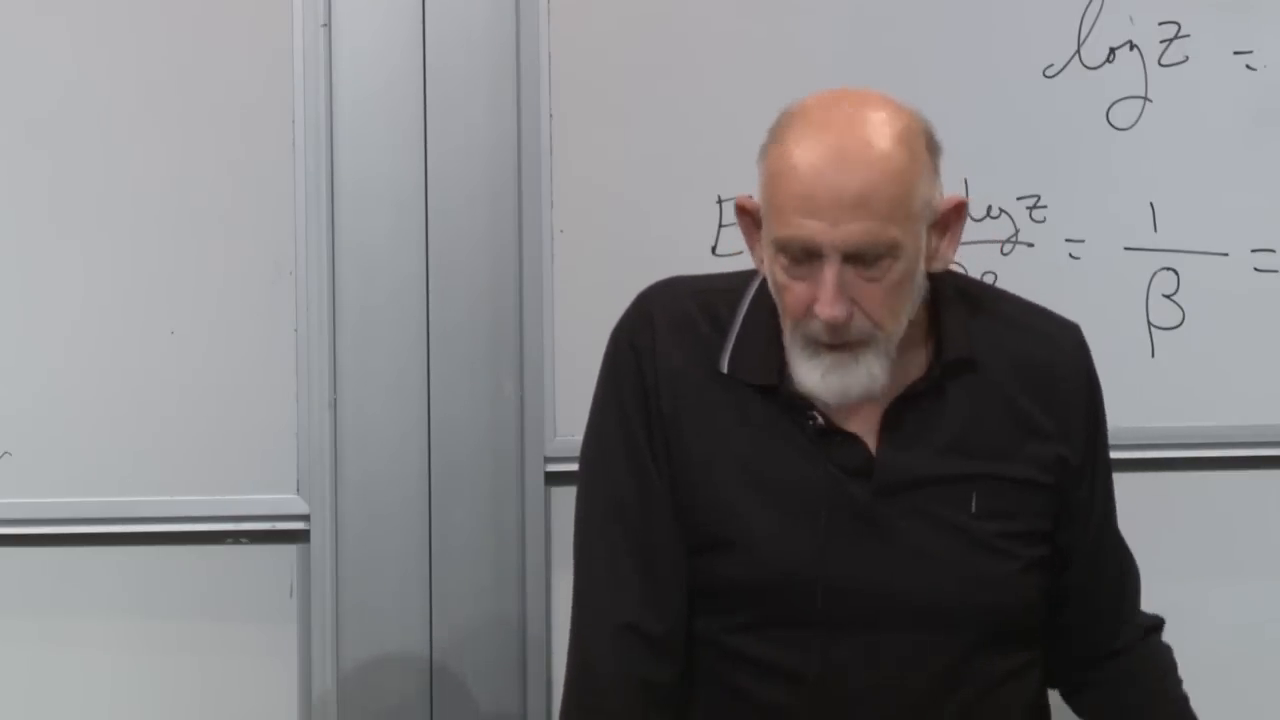
\includegraphics[width=0.90\textwidth]{lecture_07_figure_03.png}
\caption{Оценка для комнатного воздуха с использованием постоянной Больцмана, эффективной молекулярной массы около \(30\) протонных масс и \(T\simeq300\ {\rm K}\).}
\lectureframe{00:10:55}
\end{figure}

Задолго до появления микроскопического описания скорость звука можно было определять по измерениям зависимости давления от плотности. Статистический аргумент добавляет поразительную интерпретацию: получающаяся макроскопическая скорость задаётся тепловой скоростью отдельных молекул.

\begin{classroomqa}
\audiencequestion{Следует ли добавлять нейтроны к молекулярной массе, и учитывает ли число \(14\) для азота только протоны?}
\lecturerresponse{Указанная атомная масса уже учитывает протоны и нейтроны. Молекулярный азот содержит два атома с атомной массой около \(14\), так что его масса составляет примерно \(28\) протонных масс; для этой оценки достаточно округлить \(28\) до \(30\).
\lecturetimestamp{00:10:58--00:11:16}}
\end{classroomqa}

\begin{classroomqa}
\audiencequestion{Множитель \(3\) появился из трёх поступательных направлений, тогда как звук распространяется вдоль одного направления. Не должно ли это убрать множитель \(3\)?}
\lecturerresponse{Это справедливо предупреждает нас, что не следует отождествлять трёхмерную среднеквадратичную молекулярную скорость с одномерной скоростью распространения. Исходный довод был лишь картиной на уровне порядка величины. Корректный ответ даёт производная давления вместе с термодинамическим условием, подходящим для данной волны.
\lecturetimestamp{00:11:12--00:12:00}}
\end{classroomqa}

\begin{classroomqa}
\audiencequestion{Предполагала ли эта производная, что во время волны температура остаётся постоянной?}
\lecturerresponse{Да, показанная подстановка для идеального газа именно это и предполагала. Фиксировать температуру — правдоподобная предварительная оценка для очень малого возмущения; стандартное уточнение состоит в том, что обычный звук приблизительно адиабатичен, и тогда изотермическая производная заменяется на \(\left(\partial P/\partial\rho_m\right)_S\).
\lecturetimestamp{00:12:59--00:14:01}}
\end{classroomqa}

\begin{classroomqa}
\audiencequestion{Если изменения давления и плотности оба малы, делает ли это их производную малой?}
\lecturerresponse{Нет. Производная — это отношение двух малых изменений в бесконечно малом пределе. И \(\delta P\), и \(\delta\rho\) могут быть малы, тогда как \(\delta P/\delta\rho\) остаётся конечным и задаёт скорость волны.
\lecturetimestamp{00:14:03--00:14:23}}
\end{classroomqa}

\begin{classroomqa}
\audiencequestion{Должна ли скорость звука возрастать при сжатии газа, как это происходит при переходе от газа к жидкости или твёрдому телу?}
\lecturerresponse{Да. Производная вычисляется в рассматриваемом состоянии, и \(P(\rho,T)\) не обязана оставаться линейной. Когда молекулы оказываются тесно сжаты, уравнение состояния становится неидеальным, и \(\partial P/\partial\rho\) может существенно возрасти.
\lecturetimestamp{00:14:25--00:15:13}}
\end{classroomqa}

\begin{classroomqa}
\audiencequestion{Можно ли значение \(500\ {\rm m\,s^{-1}}\) использовать при любом давлении?}
\lecturerresponse{Нет. Оно относится к области малых плотностей, где уравнение идеального газа служит полезным приближением. Как только в \(P(\rho,T)\) входят более высокие степени плотности, производная и, следовательно, скорость звука зависят от давления и плотности.
\lecturetimestamp{00:15:14--00:16:29}}
\end{classroomqa}

\begin{classroomqa}
\audiencequestion{Перестаёт ли работать и исходная картина, в которой звук распространяется примерно с молекулярной скоростью, по мере роста плотности?}
\lecturerresponse{Вероятно, да. Эта картина приспособлена к разрежённому газу. При большой плотности коллективные взаимодействия становятся всё важнее, и именно поэтому производная уравнения состояния даёт более общее описание.
\lecturetimestamp{00:16:32--00:16:53}}
\end{classroomqa}

\begin{classroomqa}
\audiencequestion{Почему массу молекулы азота записали как примерно \(30\) протонных масс, а не \(28\)?}
\lecturerresponse{Нужна лишь численная точность, соответствующая этой оценке, поэтому \(28\) было округлено до \(30\). Если разделить исходную оценку \(500\ {\rm m\,s^{-1}}\) на \(\sqrt{3}\simeq1.7\), тоже получается значение, близкое к \(300\ {\rm m\,s^{-1}}\), хотя адиабатическая производная — это корректный способ вычислить поправку.
\lecturetimestamp{00:16:54--00:17:27}}
\end{classroomqa}

\section{Один классический осциллятор в тепловой ванне}

Теперь мы заменим свободно поступательно движущуюся молекулу одним гармоническим осциллятором, а всё остальное будем рассматривать как тепловую ванну. Непосредственный образ — это масса на пружине, но модель гораздо шире. Колеблется мода электромагнитной полости; колеблются атомы в кристалле; почти всякая устойчивая система, слегка выведенная из равновесия, в ведущем приближении совершает гармоническое движение.

Если \(x\) отсчитывать от положения равновесия, а импульс, масса и коэффициент жёсткости пружины равны соответственно \(p\), \(m\) и \(\kappa\), то гамильтониан имеет вид
\begin{equation}
 H(x,p)=\frac{p^2}{2m}+\frac{\kappa x^2}{2},
 \qquad
 \omega=\sqrt{\frac{\kappa}{m}}.
 \label{eq:sm7-classical-hamiltonian}
\end{equation}
Тепловая ванна задаёт \(T\), и с этого места мы снова используем \(k_B=1\), так что \(\beta=1/T\). Осциллятор, пришедший в равновесие с комнатной средой, имеет температуру около \(300\ {\rm K}\); у осциллятора, погружённого в жидкий гелий, температура всего несколько кельвинов. Гипотетическая пружина, помещённая в центр Солнца, не уцелела бы как пружина, но этот пример ясно показывает роль окружающей среды. Больцмановский вес факторизуется:
\begin{equation}
 e^{-\beta H}
 =e^{-\beta p^2/(2m)}
  e^{-\beta\kappa x^2/2}.
 \label{eq:sm7-factorized-weight}
\end{equation}

\begin{figure}[t]
\centering
\includegraphics[width=0.90\textwidth]{lecture_07_figure_04.png}
\caption{Пружинный осциллятор и его гамильтониан как сумма кинетической и потенциальной энергий.}
\lectureframe{00:20:55}
\end{figure}

В отличие от свободного газа, интеграл по координате не просто даёт объём сосуда. Восстанавливающий потенциал взвешивает каждое смещение:
\begin{equation}
 Z_{\rm cl}
 =\frac{1}{h}\int_{-\infty}^{\infty}dp
             \int_{-\infty}^{\infty}dx\,
 e^{-\beta p^2/(2m)}
 e^{-\beta\kappa x^2/2}.
 \label{eq:sm7-classical-z}
\end{equation}
Множитель \(1/h\) делает одномерную классическую статистическую сумму безразмерной. В выкладке на доске он опущен, поскольку не зависит от \(\beta\) и не может влиять на среднюю энергию.

\begin{figure}[t]
\centering
\includegraphics[width=0.90\textwidth]{lecture_07_figure_05.png}
\caption{Классическая статистическая сумма осциллятора разложена на гауссовы интегралы по импульсу и смещению.}
\lectureframe{00:22:55}
\end{figure}

Для интеграла по импульсу положим
\begin{equation}
 q=\sqrt{\frac{\beta}{2m}}\,p,
 \qquad
 dp=\sqrt{\frac{2m}{\beta}}\,dq.
 \label{eq:sm7-p-gaussian-substitution}
\end{equation}
Для интеграла по координате положим
\begin{equation}
 y=\sqrt{\frac{\beta\kappa}{2}}\,x,
 \qquad
 dx=\sqrt{\frac{2}{\beta\kappa}}\,dy.
 \label{eq:sm7-x-gaussian-substitution}
\end{equation}
Поскольку \(\int_{-\infty}^{\infty}e^{-u^2}\,du=\sqrt{\pi}\), используемый на доске ненормированный интеграл по фазовому пространству равен
\begin{equation}
 \int dp\,dx\,e^{-\beta H}
 =\frac{2\pi}{\beta}\sqrt{\frac{m}{\kappa}}
 =\frac{2\pi}{\beta\omega}.
 \label{eq:sm7-classical-z-unnormalized}
\end{equation}
После восстановления ячейки фазового пространства получаем
\begin{equation}
 Z_{\rm cl}=\frac{2\pi}{h\beta\omega}
           =\frac{1}{\beta\hbar\omega}.
 \label{eq:sm7-classical-z-normalized}
\end{equation}

Для энергии важна только зависимость от \(\beta\):
\begin{equation}
 \begin{aligned}
 \log Z_{\rm cl}&=\text{constant}-\log\beta,\\
 \expect{H}
 &=-\frac{\partial\log Z_{\rm cl}}{\partial\beta}\\
 &=\frac{1}{\beta}=T.
 \end{aligned}
 \label{eq:sm7-classical-energy}
\end{equation}

\begin{figure}[t]
\centering
\includegraphics[width=0.90\textwidth]{lecture_07_figure_06.png}
\caption{Полная классическая цепочка на правой доске: гауссова факторизация, \(Z\propto(\beta\omega)^{-1}\) и \(\expect{H}=1/\beta=T\).}
\lectureframe{00:30:15}
\end{figure}

Множителя \(3\) нет, потому что это осциллятор в одном пространственном измерении. Остающегося множителя \(1/2\) тоже нет, потому что имеются два независимых квадратичных члена. Каждый гауссовский интеграл даёт \(T/2\):
\begin{equation}
 \expect{K}=\frac{T}{2},
 \qquad
 \expect{U}=\frac{T}{2},
 \qquad
 \expect{H}=T.
 \label{eq:sm7-equipartition-oscillator}
\end{equation}
Это равнораспределение в наиболее полезной форме: каждый независимый квадратичный член в классическом гамильтониане даёт вклад \(T/2\).

Полученный ответ не зависит ни от \(m\), ни от \(\kappa\). Само движение, однако, зависит от этих параметров:
\begin{equation}
 \expect{p^2}=mT,
 \qquad
 \expect{x^2}=\frac{T}{\kappa},
 \qquad
 \expect{\dot{x}^2}=\frac{T}{m}.
 \label{eq:sm7-classical-fluctuations}
\end{equation}
Поэтому более тяжёлая масса движется медленнее, а более жёсткая пружина имеет меньшую амплитуду, хотя средняя энергия остаётся равной \(T\).
Это начинает тревожить, когда \(\kappa\) делают фантастически большим. Пружина, слишком жёсткая, чтобы двигаться, должна выглядеть как замороженная связь, однако классическое равнораспределение всё равно приписывает ей энергию \(T\).

\begin{classroomqa}
\audiencequestion{При \(\kappa\to\infty\) статистическая сумма стремится к нулю. Как тогда всё же можно использовать её логарифм?}
\lecturerresponse{Держите \(\kappa\) конечным, но сколь угодно большим. Его вклад в \(\log Z\) аддитивен и не зависит от \(\beta\), так что производная по \(\beta\) по-прежнему даёт \(T\). Неудобство, связанное с этим предельным переходом, реально: классический расчёт внутренне согласован, но в нём отсутствует черта природы, необходимая для очень жёстких осцилляторов.
\lecturetimestamp{00:34:01--00:34:54}}
\end{classroomqa}

\begin{classroomqa}
\audiencequestion{Для статистической суммы идеального газа требовался множитель \(N!\). Должен ли быть здесь аналогичный факториал?}
\lecturerresponse{Нет. Мы изучаем один конкретно заданный осциллятор, а не переставляем \(N\) одинаковых частиц. Для многих независимых помеченных мод статистические суммы перемножаются. Фактор неразличимости относится к другой задаче подсчёта.
\lecturetimestamp{00:35:03--00:35:40}}
\end{classroomqa}

\section{Почему классическое равнораспределение обернулось кризисом}

Реальные молекулы не являются бесструктурными точками. Двухатомная молекула содержит связь, способную колебаться, а значит — внутренний осциллятор. Наивный классический подсчёт приписал бы этой моде дополнительную тепловую энергию даже при обычных температурах. В заведомо схематическом подсчёте включение одного колебательного осциллятора повышает энергию с \(3T/2\) к \(5T/2\). Точный учёт теплоёмкости должен также включать вращательные степени свободы и различать энергию и её производную по температуре. Решающий экспериментальный факт проще: жёсткие внутренние моды при низкой температуре не давали вклада, как того требовало классическое равнораспределение.

Можно либо отрицать, что молекула имеет внутреннюю структуру, что абсурдно, либо признать, что в классической механике не хватает некоторого ингредиента. Этим ингредиентом является квантовая механика. Нам нужно совсем немного: лишь то, что гармонический осциллятор имеет равноотстоящие энергетические уровни.

\section{Квантовый осциллятор}

Сначала сдвинем начало отсчёта энергии и запишем спектр возбуждений в виде
\begin{equation}
 E_n^{\rm exc}=n\hbar\omega,
 \qquad n=0,1,2,\ldots.
 \label{eq:sm7-shifted-spectrum}
\end{equation}
Теперь статистическая сумма представляет собой настоящую сумму, а не интеграл по фазовому пространству:
\begin{align}
 Z_{\rm exc}
 &=\sum_{n=0}^{\infty}e^{-\beta n\hbar\omega} \notag\\
 &=1+x+x^2+\cdots
  =\frac{1}{1-x},
 \qquad x=e^{-\beta\hbar\omega}, \notag\\
 &=\frac{1}{1-e^{-\beta\hbar\omega}}.
 \label{eq:sm7-quantum-z}
\end{align}

\begin{figure}[t]
\centering
\includegraphics[width=0.90\textwidth]{lecture_07_figure_07.png}
\caption{Равноотстоящие уровни и вычисление статистической суммы квантового осциллятора как геометрической прогрессии.}
\lectureframe{00:42:05}
\end{figure}

Дифференцирование даёт среднюю энергию возбуждения:
\begin{align}
 E_{\rm exc}
 &=-\frac{\partial\log Z_{\rm exc}}{\partial\beta}
  =-\frac{1}{Z_{\rm exc}}
    \frac{\partial Z_{\rm exc}}{\partial\beta}
 \notag\\
 &=\hbar\omega\,
   \frac{e^{-\beta\hbar\omega}}
        {1-e^{-\beta\hbar\omega}}
  =\frac{\hbar\omega}{e^{\beta\hbar\omega}-1}.
 \label{eq:sm7-quantum-energy}
\end{align}

\begin{figure}[t]
\centering
\includegraphics[width=0.90\textwidth]{lecture_07_figure_08.png}
\caption{Тепловая энергия возбуждения, полученная взятием производной по \(\beta\) от квантовой статистической суммы.}
\lectureframe{00:46:05}
\end{figure}

\subsection{Высокая температура}

Когда \(\beta\hbar\omega\ll1\),
\begin{equation}
 e^{-\beta\hbar\omega}
 =1-\beta\hbar\omega
  +O\!\left((\beta\hbar\omega)^2\right).
 \label{eq:sm7-high-t-expansion}
\end{equation}
Числитель в \eqref{eq:sm7-quantum-energy} стремится к \(\hbar\omega\), тогда как знаменатель в главном порядке равен \(\beta\hbar\omega\). Поэтому
\begin{equation}
 E_{\rm exc}\simeq\frac{1}{\beta}=T.
 \label{eq:sm7-high-t-energy}
\end{equation}
Квантовый ответ воспроизводит классическое равнораспределение, когда в тепловую энергию укладывается много межуровневых расстояний.

\subsection{Низкая температура}

Когда \(\beta\hbar\omega\gg1\), экспонента очень мала:
\begin{equation}
 E_{\rm exc}
 \simeq\hbar\omega e^{-\beta\hbar\omega}.
 \label{eq:sm7-low-t-energy}
\end{equation}
Тепловое возбуждение осциллятора экспоненциально подавлено. При сдвинутом выборе нуля энергии оно почти равно нулю; физическая энергия нулевых колебаний будет восстановлена ниже.

\begin{figure}[t]
\centering
\includegraphics[width=0.90\textwidth]{lecture_07_figure_09.png}
\caption{Низкотемпературное разложение: первое тепловое возбуждение подавлено фактором \(e^{-\beta\hbar\omega}\).}
\lectureframe{00:51:55}
\end{figure}

Переходная область возникает, когда
\begin{equation}
 \beta\hbar\omega\sim1,
 \qquad\text{or equivalently}\qquad
 T\sim\hbar\omega.
 \label{eq:sm7-crossover}
\end{equation}
У этого условия есть непосредственный смысл. Классическое равнораспределение дало бы осциллятору энергию \(T\). Квантовые эффекты становятся неизбежными, когда этот масштаб оказывается меньше расстояния между соседними уровнями. Следовательно,
\begin{equation}
\begin{aligned}
 \hbar\omega\gg T&:\quad \text{frozen and quantum},\\
 \hbar\omega\ll T&:\quad \text{active and classical}.
\end{aligned}
 \label{eq:sm7-regimes}
\end{equation}
Более жёсткая пружина имеет большее \(\omega=\sqrt{\kappa/m}\), поэтому для классического поведения ей требуется более высокая температура.

\section{Степени свободы проявляются по мере нагревания вещества}

При низкой температуре двухатомная молекула может в тепловом отношении напоминать точечную частицу, потому что колебание её жёсткой связи выморожено. Когда \(T\) возрастает и проходит через \(\hbar\omega\), колебательная мода активируется. Вращательные моды могут активироваться на меньшем масштабе; при ещё более высоких температурах проявляется больше внутреннего движения, а в конце концов происходит ионизация атома. Нагревание не просто вкладывает больше энергии в фиксированный список мод. Оно выявляет степени свободы, которые при более низкой температуре были невидимы.

Воображаемая вложенная молекула делает эту мысль нагляднее. Два атома соединены жёсткой пружиной, а один кажущийся атом сам представляет собой пару, соединённую ещё более жёсткой пружиной. При низкой \(T\) обе структуры выглядят точечными. При первом пороге появляется внешнее колебание; при втором — внутренняя структура. Сложность системы раскрывается по одному энергетическому масштабу за раз.

\begin{classroomqa}
\audiencequestion{Если осциллятор уже находится в классическом режиме, делает ли дальнейший нагрев пружину более жёсткой или изменяет её частоту?}
\lecturerresponse{Нет. Жёсткость пружины и частота остаются фиксированными. Более высокая температура приводит к большим типичным импульсам и амплитудам, а значит, и к большей энергии. Жёсткость определяет температуру, при которой классический закон начинает работать, а не приводит к зависящему от температуры увеличению жёсткости пружины.
\lecturetimestamp{01:03:17--01:05:11}}
\end{classroomqa}

\subsection{Кристаллы и удельная теплоёмкость Эйнштейна}

Кристалл содержит очень много колебательных мод. Классическое равнораспределение приписывает каждому активному осциллятору энергию порядка \(T\) и потому завышает низкотемпературную теплоёмкость. Модель Эйнштейна 1907 года рассматривала колебания кристалла квантовомеханически и показала, почему они подавлены, пока тепловая энергия не достигает их межуровневого расстояния. Более точные модели твёрдого тела допускают распределение частот мод, но принцип вымораживания уже присутствует в расчёте Эйнштейна.

\begin{classroomqa}
\audiencequestion{Была ли это именно та работа, за которую Эйнштейн получил Нобелевскую премию, и появилась ли она только после того, как квантовая механика уже установилась?}
\lecturerresponse{Нет. В нобелевской формулировке речь шла о фотоэффекте. Модель теплоёмкости была опубликована в 1907, задолго до того, как были поняты полные основания квантовой механики. Эйнштейн принял и развил ключевые квантовые идеи, хотя позднее и возражал против некоторых сторон зрелой теории.
\lecturetimestamp{00:58:38--01:03:16}}
\end{classroomqa}

\begin{classroomqa}
\audiencequestion{В классической статистической механике сумма по дискретным состояниям заменяется, по-видимому, равномерным интегралом по координате и импульсу. Чем оправдан такой подсчёт состояний?}
\lecturerresponse{Окончательное обоснование даёт квантовая механика. В высокотемпературном пределе
\[
 Z_{\rm exc}\simeq\frac{1}{\beta\hbar\omega},
\]
что в точности совпадает с безразмерным классическим результатом \eqref{eq:sm7-classical-z-normalized}. Квантовые ячейки фазового пространства переходят в классическую меру, когда межуровневое расстояние уже не разрешается.
\lecturetimestamp{00:59:38--01:03:06}}
\end{classroomqa}

\subsection{Струна содержит бесконечно много осцилляторов}

Струна скрипки или гитары разлагается на нормальные моды: основную моду, высшие гармоники и моды со всё более короткими длинами волн. Математически существует бесконечно много осцилляторных мод. Если бы классическое равнораспределение приписывало каждой из них энергию \(T\), то струна в тепловом равновесии имела бы бесконечную энергию. Квантовая механика предотвращает эту катастрофу. Моды с самыми короткими длинами волн имеют наибольшие частоты и остаются замороженными при любой конечной температуре; по мере роста \(T\) активируется всё больше мод. Та же логика позже ляжет в основу излучения абсолютно чёрного тела.

\begin{figure}[t]
\centering
\includegraphics[width=0.90\textwidth]{lecture_07_figure_10.png}
\caption{Наложение нескольких нормальных мод на струне, иллюстрирующее, почему непрерывная струна представляет собой бесконечное множество гармонических осцилляторов.}
\lectureframe{01:09:30}
\end{figure}

\begin{classroomqa}
\audiencequestion{Можно ли непосредственно наблюдать переход от квантового к классическому режиму, и может ли нагрев обратить вспять низкотемпературное поведение?}
\lecturerresponse{Да. Температурная зависимость удельной теплоёмкости кристалла делает вымораживание и последующую активацию колебательных мод отчётливо измеримыми.
\lecturetimestamp{01:09:11--01:10:13}}
\end{classroomqa}

\begin{classroomqa}
\audiencequestion{Для многих осцилляторов нужно ли для каждой моды брать статистическую сумму одного осциллятора?}
\lecturerresponse{Для независимых мод,
\[
\begin{aligned}
 Z_{\rm tot}&=\prod_j Z_j,&
 \log Z_{\rm tot}&=\sum_j\log Z_j,\\
 E_{\rm tot}&=\sum_j E_j.&&
\end{aligned}
\]
Моды с \(\hbar\omega_j\gg T\) дают экспоненциально малый тепловой вклад; моды ниже этого порога вносят заметный вклад.
\lecturetimestamp{01:10:14--01:11:00}}
\end{classroomqa}

\begin{classroomqa}
\audiencequestion{Что произошло с энергией нулевых колебаний осциллятора \(\hbar\omega/2\)?}
\lecturerresponse{Физические уровни имеют вид
\[
 E_n=\left(n+\frac12\right)\hbar\omega.
\]
Следовательно
\[
 \begin{aligned}
 Z_{\rm phys}
 &=e^{-\beta\hbar\omega/2}Z_{\rm exc},\\
 E_{\rm phys}
 &=\frac{\hbar\omega}{2}
  +\frac{\hbar\omega}{e^{\beta\hbar\omega}-1}.
 \end{aligned}
\]
Общий сдвиг не изменяет вероятностей уровней, энтропии, теплоёмкости или тепловой энергии возбуждения, но сдвигает абсолютную среднюю энергию на \(\hbar\omega/2\). Множитель в \(Z\) зависит от \(\beta\), поэтому, когда нужна абсолютная энергия, его нельзя отбрасывать.
\lecturetimestamp{01:11:08--01:11:37}}
\end{classroomqa}

\section{Второй закон как парадокс обратимости}

Теперь мы можем вернуться к обещанной проблеме. Второй закон утверждает, что обычная макроскопическая эволюция необратима и что энтропия имеет тенденцию возрастать. Микроскопическая гамильтонова эволюция обратима. Как обратимое отображение точных состояний может породить необратимый закон для макроскопических состояний?

Представим систему точкой в фазовом пространстве высокой размерности,
\[
 \Gamma=(q_1,\ldots,q_N,p_1,\ldots,p_N).
\]
Наше знание обычно не задаётся точной точкой. Предположим, что оно задаётся равномерной плотностью вероятности на компактной области \(A\) объёма \(\Omega_A\):
\begin{equation}
 f(\Gamma)=
 \begin{cases}
  1/\Omega_A,&\Gamma\in A,\\
  0,&\Gamma\notin A.
 \end{cases}
 \label{eq:sm7-uniform-blob}
\end{equation}
В единицах, где \(k_B=1\), её мелкозернистая энтропия Гиббса равна
\begin{equation}
 S_{\rm fine}
 =-\int d\Gamma\,f\log f
 =\log\Omega_A.
 \label{eq:sm7-blob-entropy}
\end{equation}
Меньшая область означает больше информации и меньшую энтропию. Это определяет знак: рост неопределённости увеличивает занятую область и повышает \(\log\Omega_A\).

\begin{figure}[t]
\centering
\includegraphics[width=0.90\textwidth]{lecture_07_figure_11.png}
\caption{Компактная вероятностная область в схематическом двумерном сечении полного фазового пространства координат и импульсов.}
\lectureframe{01:20:20}
\end{figure}

\begin{classroomqa}
\audiencequestion{Физически ли система ограничена тем, что должна оставаться внутри нарисованной области, и находится ли она уже в равновесии?}
\lecturerresponse{Нет. Эта область описывает то, что известно о начальном состоянии, а не стенку в фазовом пространстве. Она не обязана быть равновесным распределением. Газ, первоначально заключённый в баке в одном углу комнаты, — конкретный пример специальной неравновесной информации.
\lecturetimestamp{01:14:55--01:15:24}}
\end{classroomqa}

\section{Поток Лиувилля и рост при грубом зернении}

Теорема Лиувилля утверждает, что гамильтонов поток сохраняет фазовый объём. Точная область может смещаться, растягиваться, складываться и становиться чрезвычайно тонкой, но
\begin{equation}
 \Omega_{A(t)}=\Omega_{A(0)},
 \qquad
 S_{\rm fine}(t)=S_{\rm fine}(0).
 \label{eq:sm7-liouville}
\end{equation}
Дискретный аналог — обратимая перестановка состояний. Если вначале известно, что игральная кость находится в одном из двух состояний, то взаимно-однозначная эволюция может изменить, какие именно это два состояния, но не число возможностей.

Реальные описания имеют конечное разрешение. Квантовая механика задаёт естественную ячейку фазового пространства, а классический эксперимент обладает конечной точностью измерений даже без обращения к квантовой теории. Под действием гамильтонова потока область может превратиться в длинную тонкую змейку. Если расстояние между соседними складками становится меньше масштаба разрешения, мы заменяем каждую неразрешённую окрестность грубой ячейкой. Точный занятый объём остаётся неизменным, но объединение грубых ячеек растёт:
\begin{equation}
 \Omega_{\rm coarse}(t)\geq\Omega_{A(t)},
 \qquad
 S_{\rm coarse}(t)=\log\Omega_{\rm coarse}(t).
 \label{eq:sm7-coarse-entropy}
\end{equation}

\begin{figure}[t]
\centering
\includegraphics[width=0.90\textwidth]{lecture_07_figure_12.png}
\caption{Объёмосохраняющий филамент, рассматриваемый через ячейки конечного разрешения. Точный чёрный филамент сохраняет свою площадь; красные грубые ячейки занимают большую эффективную область.}
\lectureframe{01:22:10}
\end{figure}

\begin{classroomqa}
\audiencequestion{Грубые ячейки перекрываются. Не нарушает ли это теорему Лиувилля?}
\lecturerresponse{Нет. Теорема Лиувилля относится к точному филаменту, который по-прежнему описывается взаимно-однозначной объёмосохраняющей эволюцией. Перекрытие относится к нашему размытому описанию: мы отбросили информацию о том, какая из тонких нитей содержит состояние.
\lecturetimestamp{01:21:32--01:21:50}}
\end{classroomqa}

Полезная аналогия — вата. Суммарный материальный объём всех волокон может оставаться почти постоянным, тогда как распушённый комок занимает большой кажущийся объём для наблюдателя, не способного различить отдельные волокна. Аналогично область в фазовом пространстве отращивает всё более тонкие щупальца; у них, в свою очередь, возникают ещё более тонкие щупальца. Любое фиксированное конечное разрешение рано или поздно перестаёт их отслеживать.

\begin{classroomqa}
\audiencequestion{Получается, что в классике энтропия лишь кажется возрастающей, а квантовая механика делает этот рост реальным, вводя фундаментальный предел разрешения?}
\lecturerresponse{Аргумент с грубым зернением не требует квантового предела. Энтропия относится одновременно к системе и к тем макроскопическим различиям, которые сохраняются в её описании. При бесконечной микроскопической информации мелкозернистая энтропия постоянна; при любом фиксированном конечном разрешении хаотические филаменты со временем становятся неразличимыми, и грубозернистая энтропия возрастает.
\lecturetimestamp{01:24:04--01:25:20}}
\end{classroomqa}

\section{Хаос, конечная доступная область и установление равновесия}

Для газа в ящике координаты ограничены. При фиксированной конечной полной энергии импульсы тоже ограничены, даже если вся энергия на мгновение сосредоточена в одной частице. Поэтому при обычных предположениях об ограниченности системы динамически доступная энергетическая оболочка имеет конечную меру.

\begin{figure}[t]
\centering
\includegraphics[width=0.90\textwidth]{lecture_07_figure_13.png}
\caption{Ограниченная доступная область фазового пространства рядом с филаментом и его грубозернистым представлением.}
\lectureframe{01:28:10}
\end{figure}

Близкие начальные точки в хаотической системе некоторое время проходят сходные истории, а затем расходятся. При разбое в бильярде незаметное изменение направления битка воспроизводится в последующих соударениях; различия накапливаются, пока конечные конфигурации не перестают быть связанными друг с другом. Поэтому вся начальная область растягивается и складывается по всей доступной области. При конечном разрешении она приближается к широкому, почти однородному равновесному описанию.

\begin{figure}[t]
\centering
\includegraphics[width=0.90\textwidth]{lecture_07_figure_14.png}
\caption{Компактное специальное состояние эволюционировало в сложный филамент, протянувшийся по ограниченной доступной области, тогда как грубозернистые ячейки распространились по гораздо большей площади.}
\lectureframe{01:33:10}
\end{figure}

Важны две оговорки. Сам по себе хаос не доказывает, что каждая траектория посещает любую доступную окрестность; для этого более сильного утверждения требуется эргодичность или свойство перемешивания. И не всякая физическая система хаотична. Типичный многочастичный газ и идеализированные бильярды дают именно ту постановку, которая здесь имеется в виду, где перемешивание является полезным физическим ожиданием.

\section{Возврат не отменяет необратимости}

Предположим, что все молекулы воздуха сначала находятся в одном углу и имеют специально подготовленную конфигурацию скоростей. Столкновения быстро распределяют их по комнате, и грубозернистое описание достигает равновесия. В фазовом пространстве с конечной мерой, сохраняемой эволюцией, теорема Пуанкаре о возврате утверждает, что почти всякая начальная точка возвращается сколь угодно близко к своей исходной точке. При допуске \(\epsilon>0\) время возврата \(t_R(\epsilon)\) конечно при выполнении гипотез теоремы, хотя для макроскопической системы оно фантастически велико. Точный возврат в бесконечно точно заданную точку не требуется и, вообще говоря, не ожидается.

\begin{classroomqa}
\audiencequestion{В примере с бильярдом не вносит ли удар по битку энергию и не нарушает ли этим замкнутую эволюцию?}
\lecturerresponse{Выбранное начальное состояние задаётся сразу после удара, когда эта энергия уже учтена. Возврат относится к последующей изолированной динамике идеализированного бильярда; возврат вблизи начального состояния включает конфигурацию, эквивалентную тому, что биток приближается к пирамиде в пределах выбранного допуска.
\lecturetimestamp{01:35:37--01:35:55}}
\end{classroomqa}

\begin{classroomqa}
\audiencequestion{Если газ в конце концов может вернуться в угол, значит ли это, что мы потеряли информацию, и действительно ли система обратима?}
\lecturerresponse{Микроскопическая динамика всё время остаётся обратимой. Грубозернистая энтропия может возрастать, потому что мы перестаём различать тонкие корреляции, и всё же исключительно редкая флуктуация может вернуть систему вблизи её особого начального макросостояния. Следовательно, возврат и грубозернистая необратимость совместимы.
\lecturetimestamp{01:37:34--01:38:15}}
\end{classroomqa}

Это приводит к существенной формулировке Больцмана. Энтропия не возрастает в каждый логически возможный момент. Для неравновесного макросостояния большой системы подавляюще больше совместимых микроскопических продолжений ведут к более крупным макросостояниям, чем к ещё более специальным. Энтропия \emph{вероятно} возрастает. Нисходящие флуктуации и возвраты допустимы, но их вероятности и временные масштабы делают их невидимыми в обычном макроскопическом опыте. Проблема обратимости была одной из великих исторических проблем статистической механики и тяжело давила на Больцмана. Эту историческую связь не следует превращать в простое причинное утверждение о его жизни.

\section{Что означает хаос}

Для более операционального определения хаоса предположим, что две начальные точки фазового пространства различаются на \(\delta\Gamma(0)\); тогда в хаотическом направлении обычно имеет место
\begin{equation}
 \lVert\delta\Gamma(t)\rVert
 \sim e^{\lambda t}\lVert\delta\Gamma(0)\rVert,
 \qquad \lambda>0,
 \label{eq:sm7-lyapunov-growth}
\end{equation}
в том режиме, где осмысленно линеаризованное расхождение. Число \(\lambda\) — показатель Ляпунова. Чтобы предсказывать для времени \(t\), требуемая точность начальных данных масштабируется примерно как \(e^{-\lambda t}\). Точность задания динамического закона тоже важна: ошибки модели усиливаются вместе с ошибками в начальных условиях. Погода — привычный пример.

\begin{classroomqa}
\audiencequestion{Существует ли принцип, утверждающий, что \emph{большинство} систем хаотичны, или это лишь эмпирическое наблюдение?}
\lecturerresponse{Существует бесконечно много хаотических и нехаотических гамильтонианов, и даже слово \emph{большинство} требует меры на пространстве гамильтонианов. Сложные взаимодействующие системы часто хаотичны, но простого универсального теста, который позволял бы при простом рассмотрении классифицировать любой гамильтониан, не существует.
\lecturetimestamp{01:39:27--01:40:49}}
\end{classroomqa}

\begin{classroomqa}
\audiencequestion{Что именно означает слово \emph{хаотический} в этом обсуждении?}
\lecturerresponse{Близкие фазовые траектории расходятся достаточно быстро, так что для долговременного предсказания требуется экспоненциально растущая точность задания начальных условий. Гармонический осциллятор служит контрастным примером: соседние фазовые точки вращаются вместе и остаются близкими. Точная задача Кеплера двух тел также нехаотична, тогда как общая задача трёх тел имеет хаотические режимы.
\lecturetimestamp{01:40:50--01:43:45}}
\end{classroomqa}

\begin{classroomqa}
\audiencequestion{Должны ли законы движения, как и начальные условия, быть известны с высокой точностью?}
\lecturerresponse{Да. Оба источника ошибок проходят через динамику, и хаотическая эволюция усиливает оба.
\lecturetimestamp{01:43:46--01:43:55}}
\end{classroomqa}

Двойной маятник даёт наглядный пример. Обычный маятник интегрируем и предсказуем. Если добавить второй маятник, то траектории, начинающиеся почти вместе, со временем могут по-разному передавать энергию и направиться в совершенно разные стороны.

\begin{figure}[t]
\centering
\includegraphics[width=0.90\textwidth]{lecture_07_figure_15.png}
\caption{Двойной маятник как конкретный пример детерминированного хаоса.}
\lectureframe{01:44:40}
\end{figure}

\begin{classroomqa}
\audiencequestion{Почему одна механическая система может быть хаотической, а другая — нет?}
\lecturerresponse{Это свойство гамильтониана и его инвариантных структур, а не следствие трения или экспериментального шума. Математически установить это может быть трудно; сложность наводит на мысль, но не является доказательством.
\lecturetimestamp{01:44:03--01:45:58}}
\end{classroomqa}

\begin{classroomqa}
\audiencequestion{Остаётся ли идеальный двойной маятник хаотическим при отсутствии трения?}
\lecturerresponse{Да. Диссипация не требуется. Точное детерминированное гамильтоново движение может обладать чувствительной зависимостью от начальных условий. Начальные данные бесконечной точности определяли бы траекторию неограниченно долго, но конечная точность даёт конечный горизонт предсказуемости.
\lecturetimestamp{01:45:57--01:47:54}}
\end{classroomqa}

\begin{classroomqa}
\audiencequestion{Совпадает ли хаос с отсутствием решения в замкнутой форме?}
\lecturerresponse{Нет. У хаотических систем, как правило, нет глобально полезного выражения траектории в замкнутой форме, но аналитическая разрешимость и чувствительная зависимость — разные свойства. Хаос диагностируется динамически по расхождению траекторий, а не просто нашей неспособностью записать формулу.
\lecturetimestamp{01:48:20--01:49:23}}
\end{classroomqa}

\begin{classroomqa}
\audiencequestion{Чем широко распространённый хаос отличается от точного удержания равновесия на неустойчивой вершине холма?}
\lecturerresponse{Вершина холма — одно исключительное неустойчивое состояние: вдали от неё близкие траектории не обязаны быстро расходиться. В хаотической области неустойчивость типична вдоль орбиты, и близкие фазовые точки многократно расходятся. Положительный показатель Ляпунова характеризует это постоянное нарастание.
\lecturetimestamp{01:49:27--01:50:11}}
\end{classroomqa}

\section{От микроскопического движения к статистическому закону}

Оценка скорости звука показала, как микроскопическое тепловое движение задаёт макроскопический масштаб распространения, а вопросы выявили, какую именно термодинамическую производную нужно указать. Затем осциллятор показал, где классическое равнораспределение применимо, а где оно не работает. Квантовое расстояние между уровнями замораживает жёсткие моды, объясняет, почему теплоёмкости меняются с температурой, и не позволяет бесконечно многим высокочастотным модам нести бесконечную тепловую энергию.

Тот же переход от точной микрофизики к эффективному макроскопическому описанию разрешает кажущееся противоречие, лежащее в основе второго начала. Гамильтонов поток сохраняет точный объём фазового пространства и остаётся обратимым. Хаотическое растяжение создаёт более тонкие корреляции, чем сохраняет макроскопическое описание, поэтому в огрублённом описании занятая область растёт. Возвратность гарантирует, что редкие возвращения не запрещены; вероятность объясняет, почему они не определяют обычный опыт. Второе начало — не новая необратимая микроскопическая сила. Это чрезвычайно надёжное статистическое направление эволюции для специальных макроскопических начальных условий в системах с огромным числом степеней свободы.